\section{Directory-Based Coherence}
%

Let's begin our journey with the classic proverb

\say{The devil is in the details.}


\vspace{1mm}

\noindent The snooping protocol can become messy! write and
upgrade misses are not atomic in any recent multiprocessor. The steps of detecting a write or upgrade miss, communicating with the other processors and
memory, getting the most recent value for a write miss and ensuring that any
invalidates are processed, and updating the cache cannot be done as though they
took a single cycle.

\noindent In a multi-core with a single bus, these steps can be made effectively atomic by
arbitrating for the bus to the shared cache or memory first (before changing the
cache state) and not releasing the bus until all actions are complete. However, the demand for higher bandwidth makes the use of only one bus impractical. Synchronizing multiple buses requires extra effort and proves quite costly for multi-processors with too many processors.

\vspace{1cm}
Our goal is to examine different ideas from the past to overcome the issue of complexity. The main references of this section are the source book and \href{https://course.ece.cmu.edu/~ece447/s15/lib/exe/fetch.php?media=censier.pdf}{this paper}.



\begin{figure}[h]
    \centering
    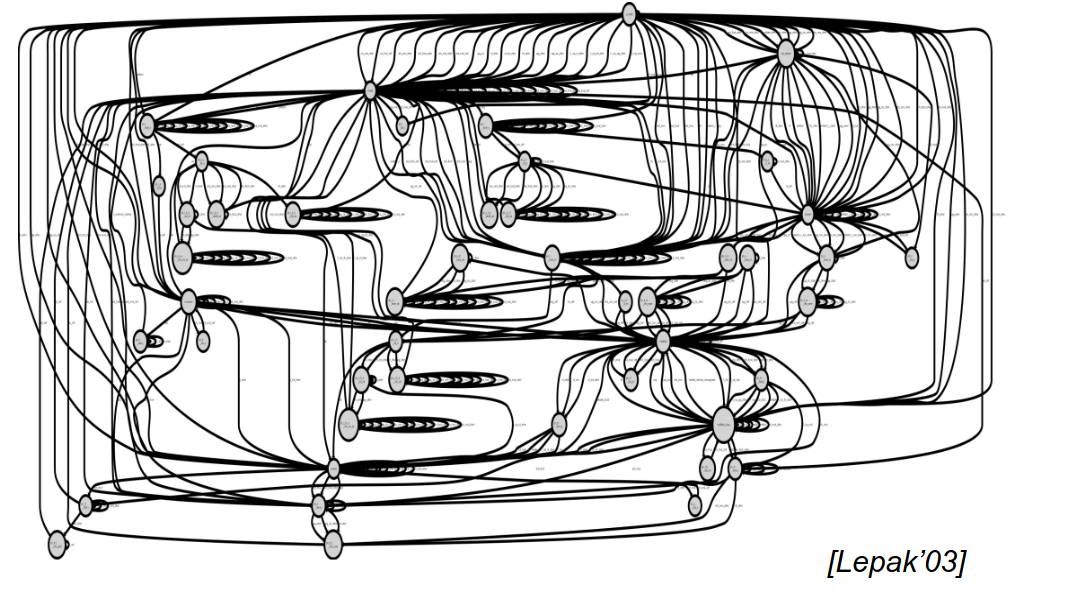
\includegraphics[width=0.75\textwidth]{snoop_bus.png}
    \caption{State Diagram of Snooping Bus (L2 MOETSI)}
    \label{fig:enter-label}
\end{figure}


The concept of cache memory was initially investigated by processors such as Atlas2 and IBM System/360 Model 85. In cache memory, the address of data corresponds to that in the main memory. However, due to limited capacity, caches can only hold a fraction of the total memory capacity. When a processor requests data and finds it in its cache, it registers a 'hit.' If not found, it results in a 'miss,' requiring data to be copied from the main memory to the cache (in a non-store-through mode). The process of checking the presence of a block in the cache is done by a directory associated to the cache which holds data like \textbf{tag} or \textbf{per cache flags} like \textbf{valid} flag.

For the sake of simplification, let's consider a scenario wherein there exists a single shared bus among processors. Moreover, the cache replacement policy implemented will prioritize the least used data.

\vspace{1cm}

\textbf{a)} \textbf{Base approach (The Classic Solution in the Paper): }

\vspace{1mm}

Broadcast each modification to all other cores. If data is present in other caches, then the core resets the valid bit of the block in the directory.

\vspace{1mm}

1) Draw an FSM chart for the state of each block in this model.

\vspace{1mm}

2) What are the weak points of this approach? (check unnecessary broadcasts, main memory access for update and ...)

\vspace{1mm}

3) Assume each broadcast consumes $\alpha \text{ energy unit}$, each access to memory consumes $\beta \text{ energy unit}$ and each access to directory consumes $\gamma \text{ energy unit}$. 

\begin{figure}[!h]
    \centering
    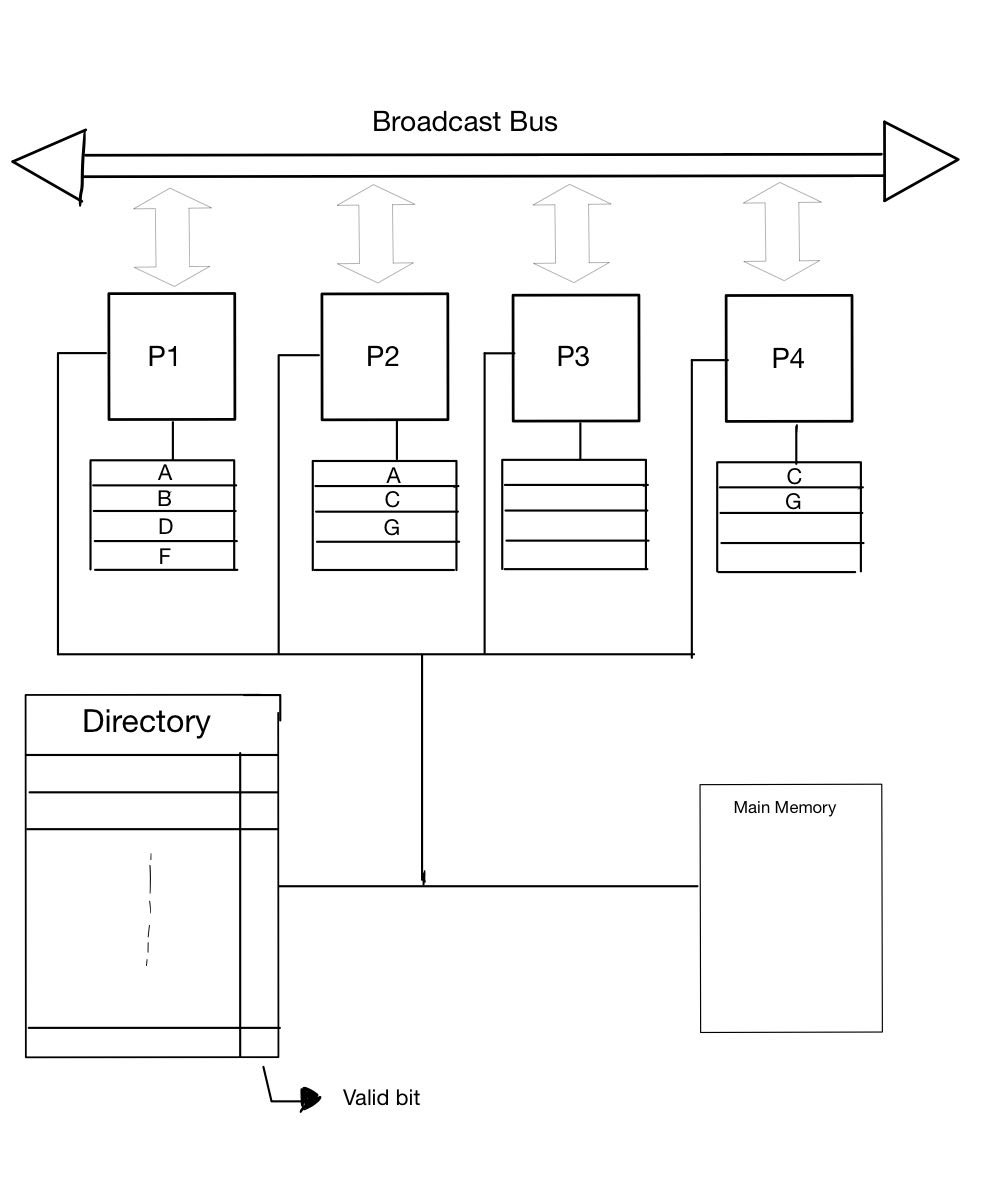
\includegraphics[scale=0.23]{5_a.png}
    \caption{\textbf{Multi-Cache System}. Each Processor has a private cache.}
    \label{fig:enter-label}
\end{figure}


Calculate the energy consumption of broadcasting and updating of directory or memory after running the following instructions (Consider the initial state of the system). Determine the valid bit of each cache block.


\begin{verbatim}
Executed Memory instructions:
load  A \\ P1
load  A \\ p2
store A \\ p1
load  A \\ p3
load  G \\ p2
store B \\ P2
store F \\ p1
\end{verbatim}


\textbf{b) }We will augment the directory by including four \textbf{presence bits} for each block. Each bit will indicate the availability of the block in a specific processor. For instance, if the presence bits for block 'A' are represented as 0010, it signifies that the block is solely present in processor P2. 

\noindent we also add a private bit to each block in the caches which indicates that the block is only available in this cache.

\noindent With the inclusion of these presence bits, broadcasting an invalid signal to other processors becomes unnecessary when a block is private. In the event another processor attempts to access a private block, the private bit will be reset. It's essential to note that any write operation by a core on a block will mandate an update to the main memory. Additionally, an invalid signal will be broadcasted only if the block is not private. 

\vspace{1mm}

1) Add \textbf{presence bits} to directory for each cache block in directory and private bit to each block in caches in figure 2.


3) Execute part (a) instructions and calculate energy. 

\vspace{2cm}

\textbf{c)} To enhance the directory structure, let's incorporate a \textbf{modify flag} for each block. This particular bit will signify whether a block has been updated within an individual cache or not. Considering the high cost associated with accessing the main memory, the inclusion of this bit serves the purpose of preventing immediate updates to the main memory for private blocks unless other caches attempt to access the same block.

\noindent For instance, when reading block 'A', if the modify flag is set, the read operation will result in a miss, triggering an update of the main memory using the value stored in the cache that holds the modified data. Subsequently, the modify bit will be reset, and the presence bits will be updated accordingly. This strategy optimizes main memory updates, triggering them only when necessary due to other caches attempting to read the same block. Moreover, if a processor modifies a shared block, it triggers a reset of the presence and valid bits in other units.

1) Execute part (a) instructions and calculate energy. 


\vspace{3mm}

\textbf{d)} (OPTIONAL) The approach described earlier, with a single directory unit handling block updates and memory management, stands in contrast to snooping, which is a distributed method for managing the same issue. The tradeoff here lies in the significant memory consumption associated with the single directory unit approach. However, unlike snoopy bus protocols, this older idea has the potential to be scalable and can be implemented alongside variations of the MSI (Modified, Shared, Invalid) protocol. What configuration can benefits from both of these designs?